\documentclass[border=12pt]{standalone}
\usepackage{tikz}
\usetikzlibrary{shapes.geometric, arrows.meta, positioning, calc, fit, backgrounds}
\usepackage{fontspec}
\usepackage{amsmath,amssymb}
\setmainfont{DejaVu Sans}

\begin{document}
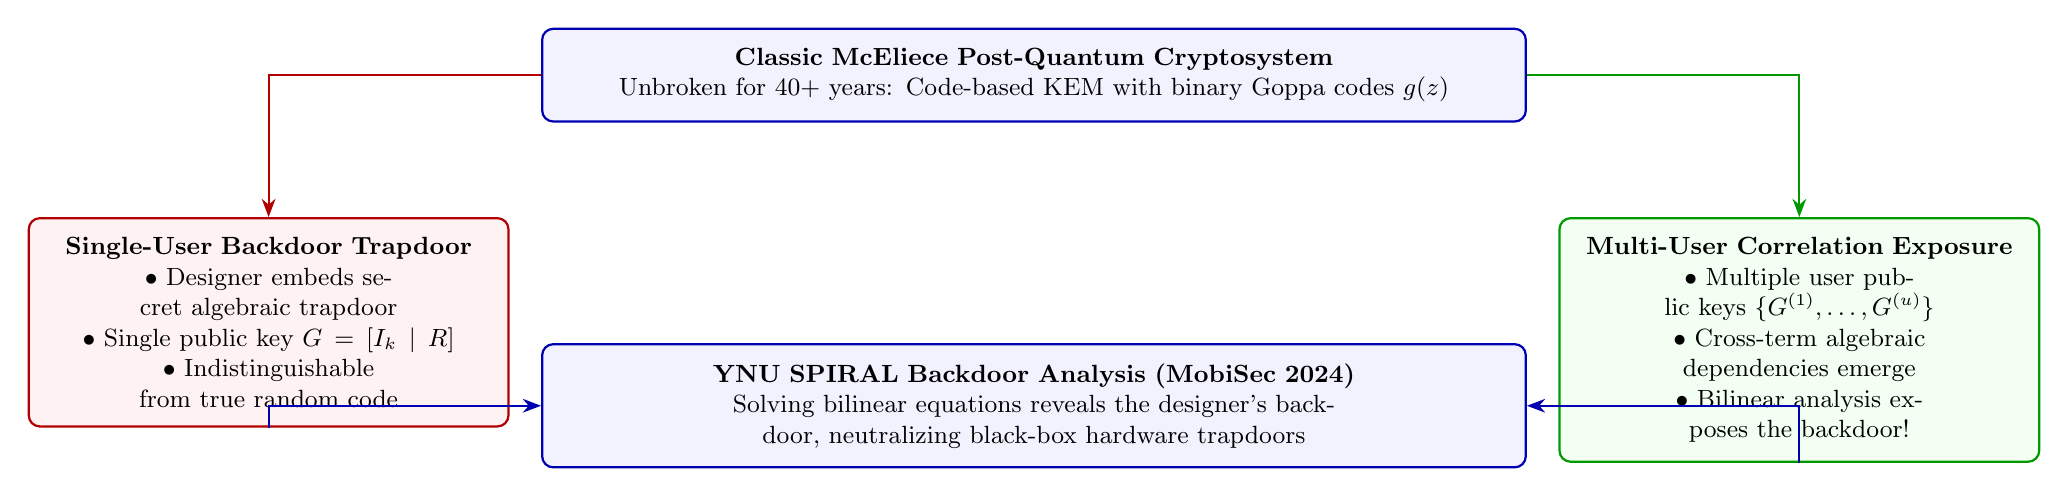
\begin{tikzpicture}[
    font=\small,
    >=Stealth,
    node distance=1.2cm,
    block/.style={rectangle, draw=blue!70!black, fill=blue!5, rounded corners=4pt, thick, align=center, inner sep=7pt},
    alertblock/.style={rectangle, draw=red!70!black, fill=red!5, rounded corners=4pt, thick, align=center, inner sep=7pt},
    greenblock/.style={rectangle, draw=green!60!black, fill=green!5, rounded corners=4pt, thick, align=center, inner sep=7pt},
    amberblock/.style={rectangle, draw=orange!80!black, fill=orange!5, rounded corners=4pt, thick, align=center, inner sep=7pt}
]

\node[block, text width=12cm] (top) {\textbf{Classic McEliece Post-Quantum Cryptosystem}\\Unbroken for 40+ years: Code-based KEM with binary Goppa codes $g(z)$};

\node[alertblock, below left=1.2cm and 0.4cm of top, text width=5.6cm] (single) {\textbf{Single-User Backdoor Trapdoor}\\$\bullet$ Designer embeds secret algebraic trapdoor\\$\bullet$ Single public key $G = [I_k \mid R]$\\$\bullet$ Indistinguishable from true random code};

\node[greenblock, below right=1.2cm and 0.4cm of top, text width=5.6cm] (multi) {\textbf{Multi-User Correlation Exposure}\\$\bullet$ Multiple user public keys $\{G^{(1)}, \dots, G^{(u)}\}$\\$\bullet$ Cross-term algebraic dependencies emerge\\$\bullet$ Bilinear analysis exposes the backdoor!};

\node[block, below=2.8cm of top, text width=12cm] (bottom) {\textbf{YNU SPIRAL Backdoor Analysis (MobiSec 2024)}\\Solving bilinear equations reveals the designer's backdoor, neutralizing black-box hardware trapdoors};

\draw[->, thick, red!70!black] (top) -| (single);
\draw[->, thick, green!60!black] (top) -| (multi);
\draw[->, thick, blue!70!black] (single) |- (bottom);
\draw[->, thick, blue!70!black] (multi) |- (bottom);

\end{tikzpicture}
\end{document}
